\documentclass[conference]{IEEEtran}
\IEEEoverridecommandlockouts
% The preceding line is only needed to identify funding in the first footnote. If that is unneeded, please comment it out.
%\usepackage{cite}
\usepackage{amsmath,amssymb,amsfonts}
\usepackage{algorithmic}
\usepackage{graphicx}
\usepackage{textcomp}
\usepackage{xcolor}
\usepackage{verbatim}
\usepackage{biblatex}

%to add images
\usepackage{graphicx}
\graphicspath{{Images/}}

\addbibresource{references.bib}

\def\BibTeX{{\rm B\kern-.05em{\sc i\kern-.025em b}\kern-.08em
    T\kern-.1667em\lower.7ex\hbox{E}\kern-.125emX}}
\begin{document}

\title{Analyzing the Influence of Various Factors on Global Economies}
%\thanks{Identify applicable funding agency here. If none, delete this.}
%}

\author{\IEEEauthorblockN{Adithi Satish}
\IEEEauthorblockA{\textit{Computer Science \& Engineering} \\
\textit{PES University}\\
Bangalore, India \\
adithisatish@pesu.pes.edu}
\and
\IEEEauthorblockN{Raksha Ramesh}
\IEEEauthorblockA{\textit{Computer Science \& Engineering} \\
\textit{PES University}\\
Bangalore, India \\
raksharamesh@pesu.pes.edu}
\and
\IEEEauthorblockN{Shriya B Shankar}
\IEEEauthorblockA{\textit{Computer Science \& Engineering} \\
\textit{PES University}\\
Bangalore, India \\
shriya.shankar19@gmail.com}
}

\maketitle

\begin{abstract}
The primary goal of this project is to use statistical analysis methods 
like multiple linear regression using ordinary least squares to gain insights 
into the numerous and diverse factors that affect economies 
of all countries globally, from quite obvious factors like 
Trade and the Finance Sector, to other parameters like Poverty, 
Gender and Urban \& Social Development, using data obtained from the 
World Bank's reserve of World Development Indicators, collected over the 
last six decades. A comparison between country groups is performed using 
the standardized regression coefficients to check for contrasts between 
developed and developing countries.

Analysis of these variables on a macroeconomic scale is imperative in 
order to gain insight on the current global scenario, 
and to see if minor improvements in any sector would lead to 
monumental change and growth overall. \\
\end{abstract}

\begin{IEEEkeywords}
macroeconomic, world development indicators, time series analysis, multiple linear regression
\end{IEEEkeywords}

\section{Introduction}

Economic growth is one of the, if not the most important criteria when measuring a country’s development. Almost all of the country’s problems can be analysed with the context of its economic growth. This economic growth has various factors that influence it’s trend; some obvious ones like: GDP per Capita, Unemployment rate, Population Growth, Government Expenditure, etc; and some not so obvious ones like: Firms with female ownership, Lending interest rate, etc.

The World Bank defines the World Development Indicators as "a compilation of relevant, high-quality, and internationally comparable statistics about global development and the fight against poverty". On a global scale, analysis of macroeconomic factors is extremely important in order to make informed decisions that can bring about urban development while improving national and global economies. The WDIs are some of the foremost features considered while doing analytics as they provide almost 1,600 time-series indicators for over 200 global economies. Some of these time-series indicators extend back to 150 years. 

Analyzing the influence that different factors have on economies in developed and developing countries is paramount to understanding what kinds of economic and social reform can be brought about. This comparison will also help to pinpoint the areas which developing nations could focus on elevating, to see an improvement in the overall economy. 

In order to quantify the economy, the GDP per capita growth (in \%) is considered, which makes the comparison easier.  Factors like trade, finance and income shares have always been considered while making any sort of inferences on the economy. However, the aim of this paper is to consider several other parameters that may contribute significantly as well, including but not limited to education and literacy rates, military expenditure, gender and urban development.



\section{Review of Literature}

\subsection{Are We on the Right Path to Achieve the Sustainable Development Goals?}
The aim of this research paper \cite{SDG}, was to analyse if the world was on the right track to achieving the targets for the Sustainable Development Goals, set by the UN in 2015, for 2030. The paper tries to forecast the scenario in 2030, using the International Futures (IF) forecasting model to do the same. The targets considered by the authors include indicators for poverty, child mortality and morbidity, undernourishment, access to safe water and sanitation, education and electricity. The datasets used for analysis and forecasting differ with each target, and have been taken from UNICEF, WHO and the World Bank's WDI datasets designated for SDG analysis.\newline
The scenario analysis was done using the SSP2, or the Shared Socioeconomic Pathways. They include five scenarios that frame potential global development trajectories and allow for cross-model collaboration.

The SSP2 scenario analysis done by the authors provided a glimpse of a moderately optimistic world in 2030 in which economies grow and convergence of low and high economic countries are prevalent. The indicator "undernourished child" showed the least improvement of only an additional 6.5\% countries, as compared to primary school completion and access to water, both of which show immense improvements, with 76\% and 72\% countries achieving the targets respectively. It also provides a country and continent wise analysis, inferring that although the SDG targets chosen may be reached by minimum 40-50\% of countries overall, African countries still fare the worst and don't achieve multiple, if any targets and are aptly termed MVCs, or Most Vulnerable Countries.

The study conclusively showed that, without considering exogenous factors, the world (i.e all 186 countries analysed) is on its way to achieve two out of the nine targets by 2030 - primary school completion and a decrease in child mortality. 

In conclusion, this paper proves to be an incredibly strong starting point, as the dataset used here and in our problem statements seem to intersect. Along with this, the target variables analysed in this study might also be very influential with respect to our problem statement at hand. In addition to this, the study also is a great reference for models like SSPs and IFs, although both have cons that would hinder their usage and application. The study also fails to consider exogenous variables, which proves to be a deterrent to the credibility of the results obtained. All in all, it can be viewed as a foundation for our analysis, giving a brief idea as to how macroeconomic and socioeconomic analysis is done, in order for us to improve, develop further and newer insights by bringing in other indicators into the foray.

\subsection{Forecasting Egyptian GDP Using ARIMA Models}\label{forcastegypt}

This paper\cite{forecastegypt}, seeks to forecast the Egyptian GDP and perform time-series analysis on the same using well known methods like the ARIMA using the Box-Jenkins approach to do the same, as well as running diagnostic tests to check for most optimal parameters and homoscedasticity of residuals. This paper uses data from the World Bank over the last 5 decades (from 1965 to 2016) for analysis and forecasting, 52 data points to be precise. 

The exploratory analysis done shows that the time-series in this case is non-stationary, and hence, differencing has to be applied to the dataset (the ARIMA model is used). The study shows that a difference factor of 2 works best in this case, converting the time-series into a stationary one. Following this, the p and q parameters are estimated using the ACF and PACF plots to each be equal to 1.
The equation for the ARIMA(1,2,1) model is found to be
\[X_t = 0.0005 + 0.1081X_{t-1} + 1.0478\epsilon_{t-1} + \epsilon_t \]


The authors performed diagnostic checks on the model, to check the normality and stationarity of the residuals obtained, in line with the Box-Jenkins approach. 

On passing all diagnostic checks and analysing the out-of-sample forecasts, the authors further infered that the Egyptian GDP is predicted to rise over the next ten years, also noting that this model is just a prediction and cannot be expected to accommodate the complex and dynamic nature of the economy. 

This paper provides a crisp analysis of one of the most common forecasting methods, ARIMA(p,d,q) used in the industry, and also highlights the interdisciplinary applications of statistical and data analysis models in real-world scenarios. The dataset used for analysis and forecasting is taken from the World Bank’s WDI GDP indicator, which reflects the data chosen for our problem statement. The methodology followed is very thorough and all parameters are taken care of, with the appropriate diagnostic checks done. However, further valuable insights could be drawn from taking other features that underline a nation’s economy into consideration and finding out the correlation between those attributes and the GDP. In conclusion, this paper provides a very clear and concise procedure that can be followed while performing time-series analysis using the ARIMA and Box-Jenkins approach.

\subsection{Factors Affecting Economic Growth in Developing Countries}\label{econgrwth}
This study employed the empirical model of economic growth proposed by Barro (1996), and used newer data to test whether the theory of economic growth that held true for most of the countries in his sample will hold true for a set of developing countries. This study attempted to find the factors that determine economic growth in developing countries.

The list of developing countries was taken from the World Bank (2015). It included the World Bank's list of low-income and lower-middle income economies.Once the data was collected, multiple Ordinary Least Squares regressions were used. This helped find the relationship between economic growth and other variables that were identified to have an impact on economic growth in previous studies. Each year was tested separately and then compared with the other years to see if the results yielded were similar.

The proxy for economic growth was the growth rate of GDP per capita, which was the dependent variable. The control variables were chosen as follows: starting level of GDP per capita, volume of exports, natural resources produced by the country, government debt, net foreign aid received, life expectancy, investment and foreign direct investment inflow into the country. The Ordinary Least Squares model used in this study was as follows: GROWTH = f (INITIALGDP, EXPORT, DEBT, RESOURCE, AID, LIFE, INVEST, FDI). 

The results were checked for multicollinearity using the variance inflation factor (VIF), which showed that the results didn’t have multicollinearity.The results showed that the increase in the volume of exports, production of natural resources, life expectancy and investment had positive effects on the economy. Therefore,to improve the economic growth of a nation, policies promoting these factors should be encouraged.

This paper gave an exemplary insight into the approach that can be employed to find a solution to  our problem statement. The detail with which the approach was explained provided us with a foundation from which we can build our own strategy upon, that pertains to our requirements. In this paper, validation was done by comparing the results of all the countries of one year to the next. We plan on employing a similar technique but instead of running the model over all the countries, we would break them up into sets of related countries (by level of development, locations, etc) and compare their results with those of the next year. We would also analyse the effect of uncommon predictors on the model and their influence on developing and developed countries. All in all, this paper tackled a very similar problem statement using a dataset that was mostly coherent with ours, serving as a context with which we can build our approach. 


\subsection{International Futures (IFs) and Integrated, Long-Term Forecasting of Global Transformations}\label{if}

This paper \cite{ifmodel} provides a thorough review of the International Futures model used by Moyer and Hedden\cite{SDG}. 
The International Futures (IFs) project focuses on 3 dimensions:

\begin{itemize}
    \item{Human Capabilities, related to development of individual capabilities, improved health, education and well-being.}
    \item{Social Systems i.e. increased transparency, inclusive democracy, better distribution and inseased capable governance}
    \item Sustainability, providing rich interactions between human systems and their environment, and protection of natural systems from human activities and outputs.
\end{itemize}

The IF forecasting broadly aims to serve as a thinking tool for the analysis of near and long-term futures which may be regional, country specific or even global, covering multiple areas of issues. IFs is one of the most widely used tools for global modelling since it facilitates interaction of data analysis, forecasting and scenario-based building functionalities. It also acts as an aide to thinking, analysis and action related to global futures.

The paper highlights the advantages of the International Futures model, namely the representation of a wide range of fundamental structures in global issue systems, as well as of the agent-driven flows that change those structures over time, the extensive data foundations of the system, its integration of important global subsystems, and its usability and transparency.

While this paper talks a great deal about IFs as a tool for analysis, it also needs to be acknowledged that the model is still in a very early stage. An IF model doesn’t wholly grasp the influencing factors during analysis. Secondly, the relationship between entities is not always known, and this could be a drawback while using IFs. For example, a country might have its own specific influencing factor which might not be visible while accounting for various trends. And lastly, we live in a dynamic world with high amounts of instability. While the past data can be extrapolated to give a fair idea of future trends, it still can’t entirely account for advancements in fields like technology, which is growing at a rapid pace. IFs are also "black-box" models, i.e. a lot of the internal parameters that they are dependent on, cannot be tweaked by the user, which in some circumstances, might have a negative effect on the predicted results. Due to these disadvantages, although IFs serve as a great model to for analysis of urban development, they do not cater to our problem statement directly.


\section{Dataset}
The World Development Indicators (WDI) is the World Bank’s premier compilation 
about relevant, credible and internationally comparable statistics to determine 
global development. It consists of enumerable indicators, encompassing measures 
of poverty, growth (in public and private sectors), education, trade and finance, 
economy, climate change, to list a few. The data provides a comparison on how 
countries and the world in general has fared over the span of almost 6 decades, 
from the 60s upto 2019 (as of now). It aims to provide a quantitative look at 
some of the issues that have been plaguing the world in recent times.

Parameters were chosen with respect to how much of an influence they may have 
on a country's economical growth and social development. The primary feature chosen
as the target variable was GDP per capita growth.

Some of the parameters considered for initial exploaratory data analysis include: 
GDP per capita growth (in \%), 
Population growth (in \%), 
Crude birth and death rates (per 1000 people), 
Unemployment (modelled ISO estimate), 
Income share held by highest, lowest 10\%, 
Government expenditure on education (\% of total government expenditure).


Given the large amount of data, dating way back to the 60s, it was correctly assumed that the data representing most of the indicators was incredibly sparse. For indicators like government expenditure on education and unemployment, there was barely any or no data recorded until the late 90s or 2000s. In addition to this, using recent data (the last two decades or so) would be able to provide much more relevant insights than data from half a century ago. In order to perform dimensionality reduction, feature selection was used to drop the attributes with more than 
70\% of the data missing. Other methods of data cleaining, like mean replacement of missing values were also used in order to make the datasets suitable for exploaratory data analysis. Certain specific values had to be manually checked and replaced, like China's GDP per capita growth for 2014 and 2015, as using other methods to estimate this data would be redundant.

\begin{comment}
\section{Initial Insights}
Before deciding on how to go about forecasting and making predictions, 
exploratory data analysis and cleaning was performed on all the datasets in order to 
understand the nature of the data. 

The indicators mentioned above were analysed and compared on a global and nation wise scale, in order to find correlations and check for trends and seasonality, along with measuring the best and worst ranked countries with regards to income inequality and education expenditure.\\
\newline
\textit{Population Growth (in \%) }: The growth of the population can play a very significant role in shaping the economy. On plotting a comparison between population of the world and India, it is seen that the population growth of the world saw a sharp increase in the 1960s, and maintained it until the mid 1970s after which there is a gradual decline. India's growth however, rose gradually up to the mid 1980s, following which there is a steeper decline than that of the world, with India's relative population growth being lesser than that of the world from the early 2010s. 

\begin{figure}[htp]
    \centering
    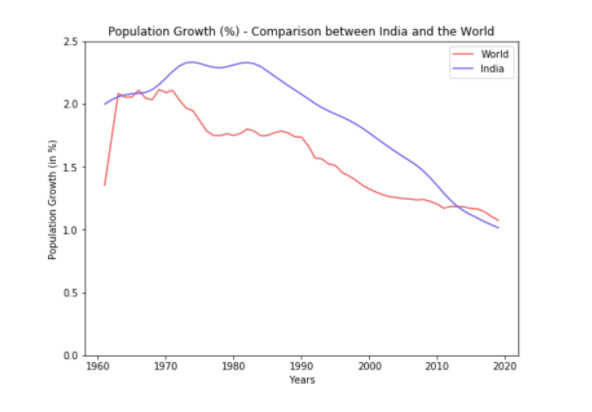
\includegraphics[width=8cm]{popGrowth1.png}
    %\caption{Caption}
    \label{fig:popGrowth}
\end{figure}

In order to find out the causes of this decline, the crude birth and death rates (per 1000 people) aggregated to represent the world were considered. The downward trend of the population growth is reflective of that of the birth and death rates as well; however the birth rate was found to be decreasing more sharply than the death rate. 

R-values for world population growth with respect to birth and death rates were found to be 0.952 and 0.745 respectively,  which solidifies the claim that the decline is population growth is more likely due to the declining birth rate rather than the death rate.\\

\textit{Unemployment}: The unemployment rate is measured as a fraction of the total labour force of a country/ the world. It is a closely watched indicator and can have a cascading effect that ripples through a country’s economy, often during recessions. The graph shows a comparison between the United States, Germany, China and India.

\begin{figure}[htp]
    \centering
    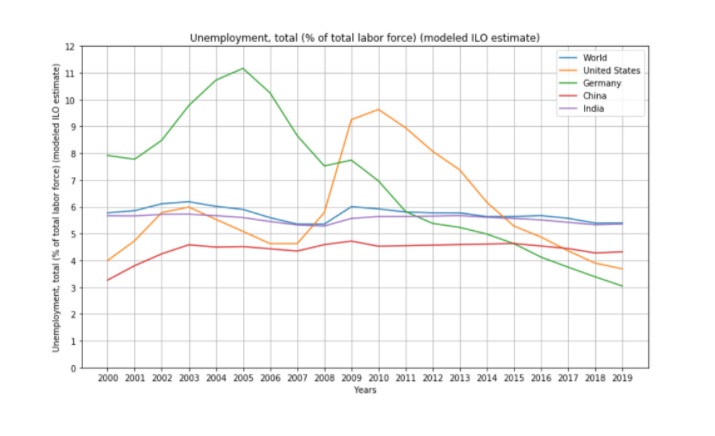
\includegraphics[width=8cm]{unemp.png}
    %\caption{Caption}
    \label{fig:unEmp}
\end{figure}

Germany seems to have fared very well when compared to the other heavy weight economies over the last fifteen years, and now has the smallest unemployment rate amongst the four, at around 3\% of its total workforce. The United States has a predictable curve, with unemployment peaking in 2009 and 2010, which followed right after the Wall Street crash of 2008. However, the rate has declined over the last ten years, standing at around 4.8\% in 2019. Unemployment rates of India, China and the world at large have remained constant over the last two decades, with India’s unemployment almost reflecting that of the world’s.\\

\textit{Income Share}: he income share held by the top and bottom 10\% of a country is a great indicator to see the disparities in the wealth distribution of the country.

To dig deeper into the income gap, the Countries where the top 10\% took the biggest income shares were compared with their own bottom 10\%.

\begin{figure}[htp]
    \centering
    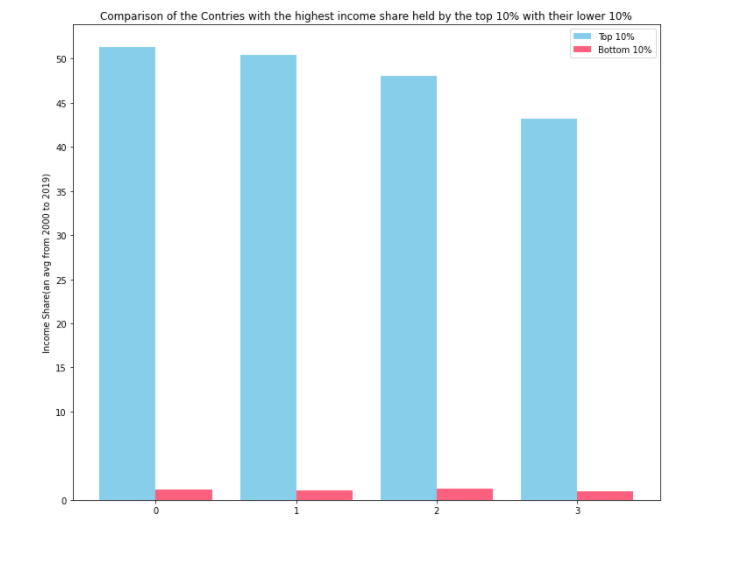
\includegraphics[width=8cm]{incComp.png}
    %\caption{Caption}
    \label{fig:my_label}
\end{figure}

It is important to notice Brazil. The Top 10\% hold close to 45\% of the income share whereas the bottom 10\% barely holds an aggregate of 1\%, which highlights the increasing wealth disparity in developing nations.\\

\textit{GDP per Capita Growth (in \%)}:  This indicator explains the growth rate of GDP per capita or the rate of increase of income per person. The following indicates the GDP per capita growth rate for India as a comparison with some of the most developed countries. There is a sharp decline around 2008-2009 for all countries which is explained by the 2008 financial crisis that took the world by storm. Despite the US being a leading contributor to the crisis, it is seen that Russia was the worst hit. Until the financial crisis, China seems to be on an exponential rise, after which the growth rate has steadied.

\begin{figure}[htp]
    \centering
    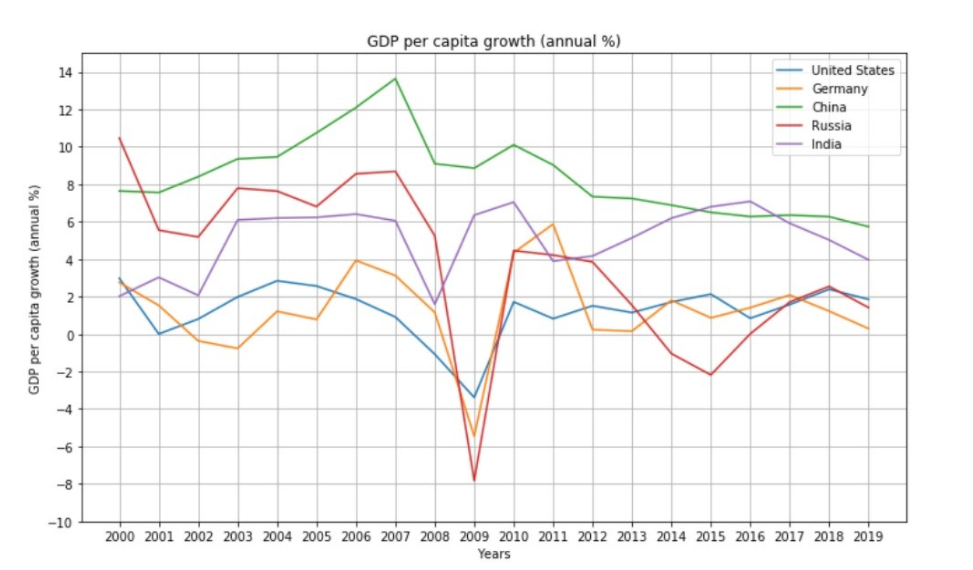
\includegraphics[width=8cm]{gdpcap.png}
    %\caption{Caption}
    \label{fig:my_label}
\end{figure}

\textit{Education expenditure (\% of government expenditure)}: It was found that the countries having the highest \% expenditure on education out of their total government expenditure are Tunisia, Ethiopia, Singapore and Ghana. A comparison was drawn between India and Singapore.

\begin{figure}[htp]
    \centering
    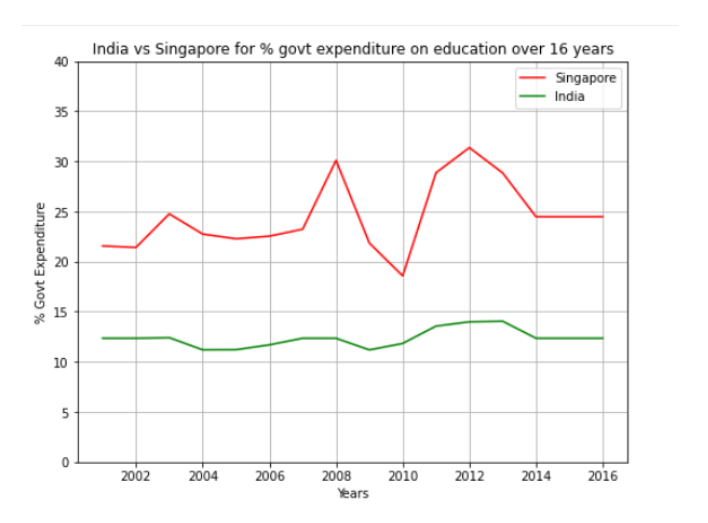
\includegraphics[width=7cm]{indsing.png}
    %\caption{Caption}
    \label{fig:my_label}
\end{figure}

Here, it can be observed that Singapore dipped drastically to ~18\% between 2008-2010 in terms of educational expenditure. However, their lowest was still far above India’s expenditure on the same. It can be seen that India has remained fairly constant within the bracket of 10-15\% in the last 2 decades.

\end{comment}


\section{Problem Statement and Proposed Solution}

On initial exploratory data analysis, the need for a comparison between countries becomes imperative. The problem statement involves measuring the influence certain parameters have had on the economy (represented here by the growth in GDP per capita) for the last few decades, for the world at large and for individual countries, and country groups. 

The dependencies of the economy on the features in developed nations, when juxtaposed with that of developing countries, is useful to provide insights as to how drastic of an effect important sectors may have on the economy. This can further be used in order to make decisions on government expenditure. 

The solution approach is to determine the impact that  parameters have on the GDP per capita growth, by subjecting these features and target variable to a Multiple Linear Regression model, using Ordinary Least Squares to estimate their respective coefficients. This needs to be done for each country in order to draw a comparison and determine which factors are more likely to influence economic activity in developed and developing nations. 

Parameters considered include population growth, income shares between the top and bottom 10\%, the unemployment rates, education as a percentage of government expenditure, military expenditure, refugee population by country of asylum/origin, financial investments, total reserves and employment grouped by gender. The target variable, as mentioned, needs to be a quantitative representative of the economy, and GDP per capita growth (in percentage) is chosen for the same. A multiple linear regression model is then modelled using these features for each country group/country, running diagnostic checks to test for accuracy, multicollinearity, homoscedasticy and normality of the residuals. The standardized beta coefficients of the regressors are compared in order to see the difference between the impacts they have on the respective GDPs. 

The na\"{i}ve assumption made is that some, if not all of these parameters, have different impacts on the economies of developed countries as opposed to developing countries. Contrasting Sub-Saharan and Asian countries with Europe and North America might provide insights as to how the GDP dependencies vary, holding in accordance with the results inferred by Moyer and Hedden \cite{SDG}, with respect to most African countries being termed MVCs (Most Vulnerable Countries) because of lack of achieving most of the Sustainable Development Goals.

Paresh Upreti\cite{econgrowth} provides an excellent starting point to begin in his paper. The analysis done in this paper, as summarized in Section \ref{econgrwth} considered features like life expectancy, foreign direct investment, foreign aid, etc. Data was taken for over 50 countries for 1995, 2000, 2005 and 2010, and subjected to multiple OLS models, in order to determine an aggregate dependence of the economy on the variables considered. However, this does not include other features like gender, military expenditure and total reserves. It also does not bring about a comparison between developed and developing nations. Additionally, this paper hasn’t explored in detail the consequences of the varying dependencies and how they can be employed to better a country’s economy. Lastly, at the time this paper was published, there wasn’t enough data available, so some of the results might not be congruent with the actual real world trends. Having better access to data, our aim is to build a more accurate model that reflects reality to a better degree.

The paper\cite{forecastegypt} summarized in Section \ref{forcastegypt} deals only with predicting Egyptian GDP using ARIMA models and does not examine the influence of any exogenous variables. It is also restricted only to forecasting one country's GDP. However, ARIMA models could be used on individual indicators like population growth and unemployment rates to see how autocorrelated they are, and forecast values for the next decade. 

Regarding IFs \cite{ifmodel}, as elaborated in Section \ref{if}, they are known to be "black-box models" and will not be very effective in the solution approach proposed above. However, they might come in handy for any future analysis that needs to be done on the indicators.

Another novel approach\cite{indchin} involved checking how far is China ahead of India, using time-series analysis, done using the same WDI dataset. The indicators considered here are trade as a percentage of GDP, Import and Export of Goods and Services, GDP per capita (adjusted by purchasing power parity), poverty alleviation, life expectancy, urban population growth, infant mortality and the adult literacy rate. Although the approach doesn't make any predictions about the dependencies of each of these factors on each other or the economy, it does provide helpful insight on how a comparison between two countries can show discrepancies in how developing nations have fared over the last few years. 

All of the papers and references reviewed provide pertinent information regarding the statistical methods used for economic analysis of this scale. However, none of them provide a country-wise comparison of the factors that hold the largest ifluence over a country's economy.


\section*{Acknowledgment}

We would like to express out profound gratitude to Dr. Gowri Srinivasa and the entire Data Analytics team, for encouraging and providing us with this opportunity to get hands-on experience in the field, and guiding us along the way. We would also like to thank the Computer Science and Engineering department at PES University, for always inspiring us to conduct frequent research and inculcating a problem-solving discipline in us.

\printbibliography

\end{document}
